\documentclass[../mathNotesPreamble]{subfiles}
\begin{document}
%  \relscale{1.4}
  \section{6.3: Volume by Slicing}

  \begin{thmBox*}[General Slicing Method]
    Suppose a solid object extends from $x=a$ to $y=b$, and the cross section of the solid perpendicular to the $x$-axis has an area given by a function $A$ that is integrable on $\sbrkt{a,b}$. The volume of the solid is
      \[V=\int_a^b A(x)\,dx.\]
  \end{thmBox*}
  \begin{center}
    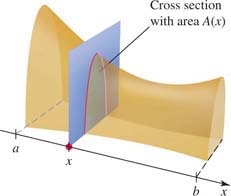
\includegraphics[width=0.22\linewidth]{../images/briggs_06_03/fig06_22}
    \hspace*{0.15\linewidth}
    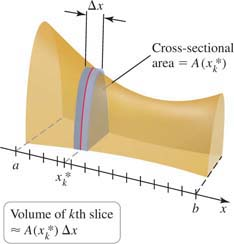
\includegraphics[width=0.22\linewidth]{../images/briggs_06_03/fig06_23}
  \end{center}

  \begin{ex*}
    Use the general slicing method to find the volume of the solid whose base is the region bounded by the semicircle $y=\sqrt{1-x^2}$ and the $x$-axis, and whose cross sections through the solid perpendicular to the $x$-axis are squares.
  \end{ex*}
  
  \begin{flushright}
    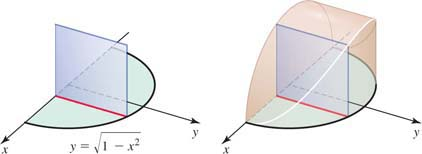
\includegraphics[width=0.4\linewidth]{../images/briggs_06_03/prac06_11}
  \end{flushright}
  \vspace*{\stretch{1}}
  \pagebreak

  \begin{thmBox*}[Disk Method about the $x$-Axis]
    Let $f$ be continuous with $f(x)\geq 0$ on the interval $\sbrkt{a,b}$. If the region $R$ bounded by the graph of $f$, the $x$-axis, and the lines $x=a$ and $x=b$ is revolved about the $x$-axis, the volume of the resulting solid of revolution is
      \[V=\int_a^b \pi\underbrace{f(x)^{\mathrlap{2}}}_{\substack{\textnormal{disk}\\\textnormal{radius}}}\,dx.\]
  \end{thmBox*}
  \vspace*{\stretch{0.5}}
  \begin{center}
    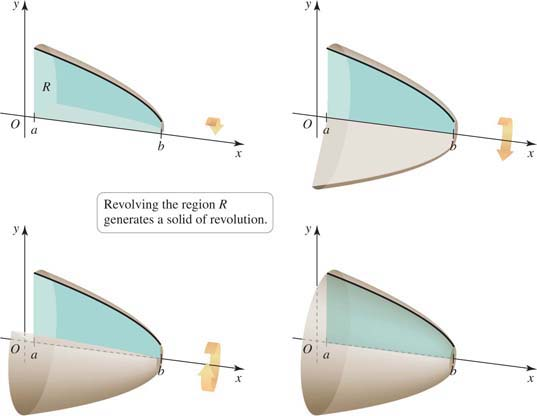
\includegraphics[width=0.4\linewidth]{../images/briggs_06_03/fig06_28}
    \hspace*{0.075\linewidth}
    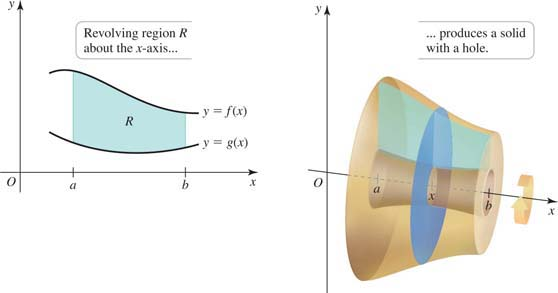
\includegraphics[width=0.45\linewidth]{../images/briggs_06_03/fig06_31}
  \end{center}
  \vspace*{\stretch{1}}

  \begin{thmBox*}[Washer Method about the $x$-Axis]
    Let $f$ and $g$ be continuous functions with $f(x)\geq g(x)\geq 0$ on $\sbrkt{a,b}$. Let $R$ be the region bounded by $y=f(x)$, $y=g(x)$, and the lines $x=a$ and $x=b$. When $R$ is revolved about the $x$-axis, the volume of the resulting solid of revolution is
      \[V=\int_a^b \pi (\underbrace{f(x)^{\mathrlap{2}}}_{\substack{\textnormal{outer}\\\textnormal{radius}}}-\underbrace{g(x)^{\mathrlap{2}}}_{\substack{\textnormal{inner}\\\textnormal{radius}}}\phantom{^2})\,dx.\]
  \end{thmBox*}
  \pagebreak

  \begin{ex*}
    Consider the region bounded by $y=e^{x/4}$, $y=0$, $x=0$, and $x=6$. Find the volume of the solid generated by rotating the region about the $x$-axis.
  \end{ex*}
  \begin{flushright}
    \begin{tikzpicture}
      \begin{axis}[
        grid style={line width=0.3pt, draw=gray!60},
        axis lines=center,
        axis line style={black,->},
        xmin=-0.75, xmax=7,
        ymin=-0.5, ymax=5.5,
        ticklabel style={font=\footnotesize,inner sep=0.5pt,fill=white,opacity=0.5, text opacity=1},
        every axis plot/.append style={line width=0.95pt, color=blue, samples=100},
        width=0.45\linewidth, height=0.3\linewidth
        ]
        \addplot[->, name path=A, ClemsonPurple] expression[domain=-0.75:7]{exp(x/4)} node[black, pos=0.5, above left] {$e^{\nicefrac{x}{4}}$};
        \addplot[draw=none, name path=B] [domain=0:6] {0};
        \addplot[fill=HowardsRock!55, opacity=0.75] fill between[of=A and B, soft clip={domain=0:6}];
      \end{axis}
    \end{tikzpicture}
  \end{flushright}
  \vspace*{\stretch{1}}
  \pagebreak

  \begin{thmBox*}[Disk and Washer Methods about the $y$-Axis]
    Let $p$ and $q$ be continuous functions with $p(y)\geq q(y)\geq 0$ on $\sbrkt{c,d}$. Let $R$ be the region bounded by $x=p(y)$, $x=q(y)$, and the lines $y=c$ and $y=d$. When $R$ is revolved around the $y$-axis, the volume of the resulting solid of revolution is given by
      \[V=\int_c^d \pi(\underbrace{p(y)^{\mathrlap{2}}}_{\substack{\textnormal{outer}\\\textnormal{radius}}}-\underbrace{q(y)^{\mathrlap{2}}}_{\substack{\textnormal{inner}\\\textnormal{radius}}}\phantom{^2})\,dy.\]
      If $q(y)=0$, the disk method results:
        \[V=\int_c^d \pi\underbrace{p(y)^{\mathrlap{2}}}_{\substack{\textnormal{disk}\\\textnormal{radius}}}\,dy.\]
  \end{thmBox*}

  \vspace*{\stretch{1}}
  \begin{center}
    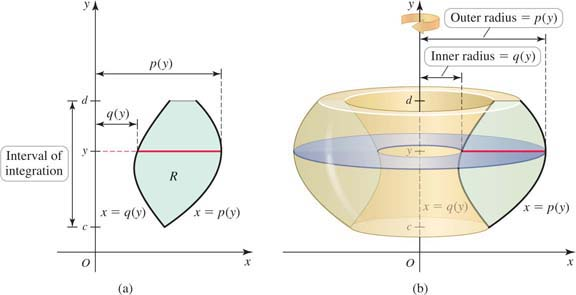
\includegraphics[width=0.7\linewidth]{../images/briggs_06_03/fig06_34}
  \end{center}
  \vspace*{\stretch{1}}
  \pagebreak

  \begin{ex*}
    Consider the region bounded between $y=\sqrt[4]{x}$, $y=2$, and $x=0$. 
  \end{ex*}
  \begin{flushright}
    \begin{tikzpicture}
      \begin{axis}[
        grid style={line width=0.3pt, draw=gray!60},
        axis lines=center,
        axis line style={black,->},
        xmin=-0.5, xmax=20,
        ymin=-0.125, ymax=2.5,
        xmajorticks=false,
        ymajorticks=false,
        ticklabel style={font=\footnotesize,inner sep=0.5pt,fill=white,opacity=0.5, text opacity=1},
        every axis plot/.append style={line width=0.95pt, color=blue, samples=100},
        width=0.45\linewidth, height=0.3\linewidth
        ]
        \addplot[->, name path=A, ClemsonOrange] expression[domain=0:20, samples=500]{x^(1/4)} node[black, pos=0.5, below right, font=\normalsize] {$y=\sqrt[4]{x}$};
        \addplot[->, name path=B, ClemsonPurple] expression[domain=0:20]{2} node[black, pos=0.5, above left, font=\normalsize] {$y=2$};
        \addplot[fill=HowardsRock!55, opacity=0.75] fill between[of=A and B, soft clip={domain=0:16}];
      \end{axis}
    \end{tikzpicture}
  \end{flushright}
  \begin{tasks}[after-item-skip=\stretch{1}, label=](1)
    \task 
      Setup the integral with respect to $x$ that gives the area of the region.
    \task 
      Setup the integral with respect to $y$ that gives the area of the region.
    \task 
      Use the disk/washer method to setup the that represents the volume of the solid generated by rotating the region about the $x$-axis.
  \end{tasks}
  \vspace*{\stretch{1}}
  \pagebreak

  \begin{ex*}
    Consider the region $R$ between $y=\sqrt{x}+1$ and $y=x^2+1$. Setup the integrals which find the volume of the solid obtained by rotating the region $R$ as indicated below.
  \end{ex*}
  \begin{flushright}
    \begin{tikzpicture}
      \begin{axis}[
        grid style={line width=0.3pt, draw=gray!60},
        axis lines=center,
        axis line style={black,->},
        xmin=-0.25, xmax=1.75,
        ymin=-0.5, ymax=2.5,
        ticklabel style={font=\footnotesize,inner sep=0.5pt,fill=white,opacity=0.5, text opacity=1},
        every axis plot/.append style={line width=0.95pt, color=blue, samples=100},
        width=0.45\linewidth, height=0.3\linewidth
        ]
        \addplot[->, name path=A, ClemsonOrange] expression[domain=0:1.2]{x^2+1} node[black, pos=0.5, below right, font=\normalsize] {$y=x^2+1$};
        \addplot[->, name path=B, ClemsonPurple] expression[domain=0:1.5]{sqrt(x)+1} node[black, pos=0.6, above left, font=\normalsize] {$y=\sqrt{x}+1$};
        \addplot[fill=HowardsRock!55, opacity=0.75] fill between[of=A and B, soft clip={domain=0:1}];
        \node[font=\normalsize] at (0.4,1.4) {$R$};
      \end{axis}
    \end{tikzpicture}
  \end{flushright}
  \begin{tasks}[after-item-skip=\stretch{1}, label=](2)
    \task 
      about the $y$-axis
    \task 
      about the $x$-axis
    \task 
      about the line $x=1$
    \task 
      about the line $y=-1$
  \end{tasks}
  \vspace*{\stretch{1}}
  \pagebreak

\end{document}
